\section{迭代算法}

\subsection{迭代法求平方根}

\begin{figure}[ht]
    \centering
    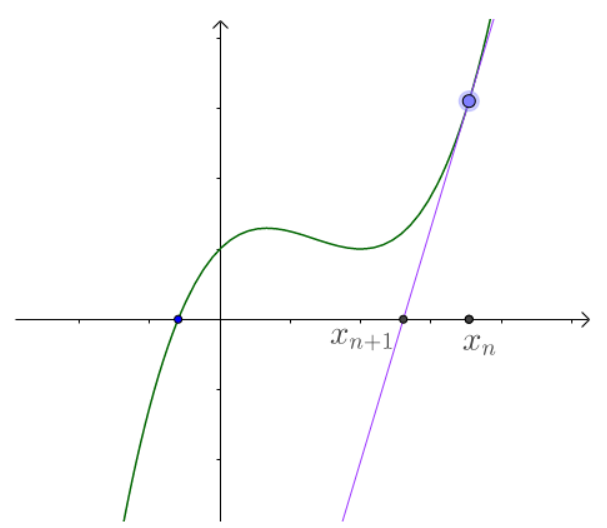
\includegraphics[width=.5\linewidth]{figures/sqrt.png}
\end{figure}

原理：

如图，一个曲线方程$f(x)$，在它的$f(x_\mathrm{n})$处画一条切线与$x$轴相交，交点为$x_\mathrm{n+1}$，如果继续在它的$f(x_\mathrm{n+1})$处画一条切线与x轴相交，会得到交点$x_\mathrm{n+2}$。而在这个过程中，可以发现交点$x_\mathrm{n+m}$会无限逼近方程$f(x)=0$的解，最终可以得到一个与理想值无限靠近的解。

而这里讨论的是求平方根，所以曲线方程更简单。比如，我们要求$N$的平方根。

那么其实就是求方程$f(x)=x^2-N$，当$f(x)=0$时方程的解。

函数$f(x)$的导函数是：$f'(x)=2x$

那么$f(x)$函数的曲线在$(x_\mathrm{n},x_\mathrm{n}^2-N)$点处切线的斜率为：$2x_\mathrm{n}$

所以切线方程为：$f(x) - (x_\mathrm{n}^2-N) = 2x_\mathrm{n}(x - x_\mathrm{n})$，即：$f(x)=2x_\mathrm{n}x - x_\mathrm{n}^2 - N$

那么切线方程与$x$轴的交点$x_\mathrm{n+1} = (x_\mathrm{n} + N/x_\mathrm{n})/2$，

我们可以将得到的交点值的平方与$N$比较，循环以上过程直到得到满意的值。

\section{递归算法}

一个函数在它的函数体内调用它自身称为递归调用，这种函数称为递归函数。执行递归函数将反复调用其自身，每调用一次就进入新的一层，当最内层的函数执行完毕后，再一层一层地由里到外退出。

阶乘 $n!$ 的计算公式如下：

$n!=\begin{cases}
    1 \quad (n = 0,1) \\
    n*(n-1)! \quad (n > 1)
\end{cases}$

根据公式编写如下的代码：
\begin{lstlisting}
    n = int(input("请输入n："))
    def factorial(n):
    if n == 0:
        return 1
    return n * factorial(n - 1)
    print(factorial(n))
\end{lstlisting}

factorial() 就是一个典型的递归函数。调用 factorial() 后即进入函数体，只有当 n==0 或 n==1 时函数才会执行结束，否则就一直调用它自身。

由于每次调用的实参为 n-1，即把 n-1 的值赋给形参 n，所以每次递归实参的值都减 1，直到最后 n-1 的值为 1 时再作递归调用，形参 n 的值也为1，递归就终止了，会逐层退出。

要想理解递归函数，重点是理解它是如何逐层进入，又是如何逐层退出的，下面我们以 5! 为例进行讲解。

{\bfseries \cgreen{递归的进入}}
\begin{enumerate}
    \item 求 5!，即调用 factorial(5)。当进入 factorial() 函数体后，由于形参 n 的值为 5，不等于 0 或 1，所以执行factorial(n-1) * n，也即执行factorial(4) * 5。为了求得这个表达式的结果，必须先调用 factorial(4)，并暂停其他操作。换句话说，在得到 factorial(4) 的结果之前，不能进行其他操作。这就是第一次递归。
    \item 调用 factorial(4) 时，实参为 4，形参 n 也为 4，不等于 0 或 1，会继续执行factorial(n-1) * n，也即执行factorial(3) * 4。为了求得这个表达式的结果，又必须先调用 factorial(3)。这就是第二次递归。
    \item 以此类推，进行四次递归调用后，实参的值为 1，会调用 factorial(1)。此时能够直接得到常量 1 的值，并把结果 return，就不需要再次调用 factorial() 函数了，递归就结束了。
\end{enumerate}

\begin{table}[ht]
    \centering
    \caption*{逐层进入的过程}
    \begin{tabular}{@{}ccccc@{}}
    \toprule
    层次/层数 & 实参/形参 & 调用形式         & 需要计算的表达式         & 需要等待的结果          \\ \midrule
    1     & n=5   & factorial(5) & factorial(4) * 5 & factorial(4) 的结果 \\
    2     & n=4   & factorial(4) & factorial(3) * 4 & factorial(3) 的结果 \\
    3     & n=3   & factorial(3) & factorial(2) * 3 & factorial(2) 的结果 \\
    4     & n=2   & factorial(2) & factorial(1) * 2 & factorial(1) 的结果 \\
    5     & n=1   & factorial(1) & 1                & 无                \\ \bottomrule
    \end{tabular}
    \end{table}

    {\bfseries \cgreen{递归的退出}}

    当递归进入到最内层的时候，递归就结束了，就开始逐层退出了，也就是逐层执行 return 语句。
    \begin{enumerate}
        \item n 的值为 1 时达到最内层，此时 return 出去的结果为 1，也即 factorial(1) 的调用结果为 1。
        \item 有了 factorial(1) 的结果，就可以返回上一层计算factorial(1) * 2的值了。此时得到的值为 2，return 出去的结果也为 2，也即 factorial(2) 的调用结果为 2。
        \item 以此类推，当得到 factorial(4) 的调用结果后，就可以返回最顶层。经计算，factorial(4) 的结果为 24，那么表达式factorial(4) * 5的结果为 120，此时 return 得到的结果也为 120，也即 factorial(5) 的调用结果为 120，这样就得到了 5! 的值。
    \end{enumerate}

\begin{table}[ht]
    \centering
    \caption*{逐层退出的过程}
    \begin{tabular}{@{}ccccc@{}}
    \toprule
    \begin{tabular}[c]{@{}c@{}}层次\\层数\end{tabular} & 调用形式         & \begin{tabular}[c]{@{}c@{}}需要计算\\的表达式\end{tabular}         & \begin{tabular}[c]{@{}c@{}}从内层递归得到的结果\\      （内层函数的返回值）\end{tabular} & \begin{tabular}[c]{@{}c@{}}表达式的值\\      （当次调用的结果）\end{tabular} \\ \midrule
    5     & factorial(1) & 1                & 无                                                                    & 1                                                              \\
    4     & factorial(2) & factorial(1) * 2 & factorial(1) 的返回值，也就是 1                                              & 2                                                              \\
    3     & factorial(3) & factorial(2) * 3 & factorial(2) 的返回值，也就是 2                                              & 6                                                              \\
    2     & factorial(4) & factorial(3) * 4 & factorial(3) 的返回值，也就是 6                                              & 24                                                             \\
    1     & factorial(5) & factorial(4) * 5 & factorial(4) 的返回值，也就是 24                                             & 120                                                            \\ \bottomrule
    \end{tabular}
    \end{table}

{\bfseries \cgreen{递归的条件}}

每一个递归函数都应该只进行有限次的递归调用，否则它就会进入死胡同，永远也不能退出了，这样的程序是没有意义的。

要想让递归函数逐层进入再逐层退出，需要解决两个方面的问题：
\begin{enumerate}
    \item 存在限制条件，当符合这个条件时递归便不再继续。对于 factorial()，当形参 n 等于 0 或 1 时，递归就结束了。
    \item 每次递归调用之后越来越接近这个限制条件。对于 factorial()，每次递归调用的实参为 n - 1，这会使得形参 n 的值逐渐减小，越来越趋近于 1 或 0。
\end{enumerate}


\subsection{二分搜索递归算法}

如何在数组中查找某一特定元素?

最low的算法：枚举

\begin{lstlisting}
lis = [1, 3, 4, 6, 7, 8, 10, 13, 14, 20, 22, 24, 30, 50, 80, 98, 100]
n = int(input("输入要查找的数:"))
for item in lis:
    if n == item:
        print("找到了")
        break
\end{lstlisting}

二分查找是一种在有序数组中查找某一特定元素的搜索算法。搜索过程从数组的中间元素开始，如果中间元素正好是要查找的元素，则搜索过程结束；如果某一特定元素大于或者小于中间元素，则在数组大于或小于中间元素的那一半中查找，而且跟开始一样从中间元素开始比较。如果在某一步骤数组为空，则代表找不到。这种搜索算法每一次比较都使搜索范围缩小一半。

\begin{figure}[htpb]
    \centering
    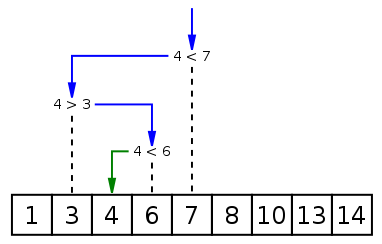
\includegraphics[width=.5\linewidth]{figures/Binary_search.png}
\end{figure}

\lstinputlisting{code/binary_search.py}

\section{分治算法}

{\bfseries \cgreen{分治算法的思想}} 

将问题规模为n的原问题归纳为规模n/2的两个子问题，或规模n/m的m个子问题；若规模缩小的子问题仍不能简单求解，则继续归约为规模更小的问题；分别求解小规模的子问题，并逐步综合得到原问题的解。

分治法所能解决的问题一般具有以下几个特征：
\begin{enumerate}
    \item 该问题的规模缩小到一定的程度就可以容易地解决
    \item 该问题可以分解为若干个规模较小的相同问题，即该问题具有最优子结构性质。
    \item 利用该问题分解出的子问题的解可以合并为该问题的解；
    \item 该问题所分解出的各个子问题是相互独立的，即子问题之间不包含公共的子子问题。
\end{enumerate}

第一条特征是绝大多数问题都可以满足的，因为问题的计算复杂性一般是随着问题规模的增加而增加；

第二条特征是应用分治法的前提它也是大多数问题可以满足的，此特征反映了递归思想的应用；

第三条特征是关键，能否利用分治法完全取决于问题是否具有第三条特征，如果具备了第一条和第二条特征，而不具备第三条特征，则可以考虑用贪心法或动态规划法。

第四条特征涉及到分治法的效率，如果各子问题是不独立的则分治法要做许多不必要的工作，重复地解公共的子问题，此时虽然可用分治法，但一般用动态规划法较好。

{\bfseries \cgreen{分治算法的解题步骤一般如下：}}
\begin{enumerate}
    \item 分解，将要解决的问题划分成若干规模较小的同类问题；
    \item 求解，当子问题划分得足够小时，用较简单的方法解决；
    \item 合并，按原问题的要求，将子问题的解逐层合并构成原问题的解。
\end{enumerate}

\begin{figure}[htpb]
    \centering
    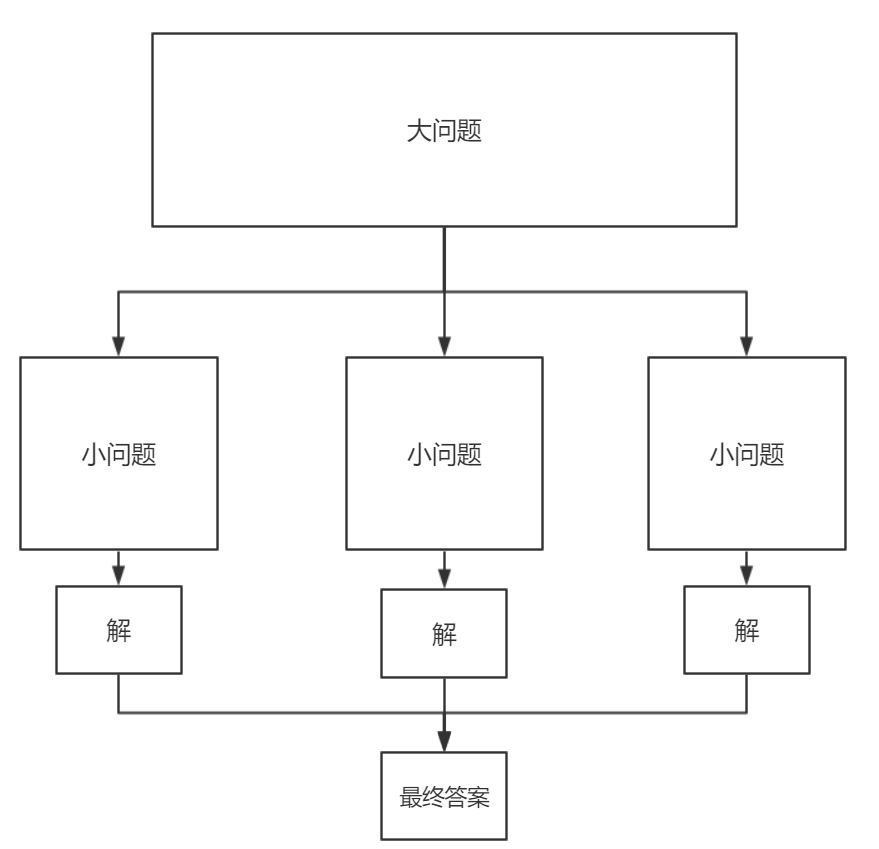
\includegraphics[width=.5\linewidth]{figures/fenzhi.png}
\end{figure}



\section{贪心算法}

\subsection{贪心算法思想}

顾名思义，贪心算法总是作出在当前看来最好的选择。也就是说贪心算法并不从整体最优考虑，它所作出的选择只是在某种意义上的局部最优选择。当然，希望贪心算法得到的最终结果也是整体最优的。虽然贪心算法不能对所有问题都得到整体最优解，但对许多问题它能产生整体最优解。如单源最短路经问题，最小生成树问题等。在一些情况下，即使贪心算法不能得到整体最优解，其最终结果却是最优解的很好近似。

\subsection{贪心算法的基本要素}

\begin{enumerate}
    \item 贪心选择
    
    所谓贪心选择是指所求问题的整体最优解可以通过一系列局部最优的选择，即贪心选择来达到。这是贪心算法可行的第一个基本要素，也是贪心算法与动态规划算法的主要区别。

    动态规划算法通常以自底向上的方式解各子问题，而贪心算法则通常以自顶向下的方式进行，以迭代的方式作出相继的贪心选择，每作一次贪心选择就将所求问题简化为规模更小的子问题。

    对于一个具体问题，要确定它是否具有贪心选择性质，必须证明每一步所作的贪心选择最终导致问题的整体最优解。
    \item 最优子结构
    
    当一个问题的最优解包含其子问题的最优解时，称此问题具有最优子结构性质。问题的最优子结构性质是该问题可用动态规划算法或贪心算法求解的关键特征。
    
    贪心算法的每一次操作都对结果产生直接影响，而动态规划则不是。贪心算法对每个子问题的解决方案都做出选择，不能回退；动态规划则会根据以前的选择结果对当前进行选择，有回退功能。动态规划主要运用于二维或三维问题，而贪心一般是一维问题。
\end{enumerate}

\subsection{贪心算法的基本思路}

贪心算法的基本思路是从问题的某一个初始解出发一步一步地进行，根据某个优化测度，每一步都要确保能获得局部最优解。每一步只考虑一个数据，他的选取应该满足局部优化的条件。若下一个数据和部分最优解连在一起不再是可行解时，就不把该数据添加到部分解中，直到把所有数据枚举完，或者不能再添加算法停止。

\begin{enumerate}
    \item 建立数学模型来描述问题；
    \item 把求解的问题分成若干个子问题；
    \item 对每一子问题求解，得到子问题的局部最优解；
    \item 把子问题的解局部最优解合成原来解问题的一个解。
\end{enumerate}

\subsection{算法特性}

\begin{itemize}
    \item 随着算法的进行，将积累起其它两个集合：一个包含已经被考虑过并被选出的候选对象，另一个包含已经被考虑过但被丢弃的候选对象。
    \item 有一个函数来检查一个候选对象的集合是否提供了问题的解答。该函数不考虑此时的解决方法是否最优。
    \item 还有一个函数检查是否一个候选对象的集合是可行的，也即是否可能往该集合上添加更多的候选对象以获得一个解。和上一个函数一样，此时不考虑解决方法的最优性。
    \item 选择函数可以指出哪一个剩余的候选对象最有希望构成问题的解。
    \item 最后，目标函数给出解的值。
    \item 为了解决问题，需要寻找一个构成解的候选对象集合，它可以优化目标函数，贪婪算法一步一步的进行。起初，算法选出的候选对象的集合为空。接下来的每一步中，根据选择函数，算法从剩余候选对象中选出最有希望构成解的对象。如果集合中加上该对象后不可行，那么该对象就被丢弃并不再考虑；否则就加到集合里。每一次都扩充集合，并检查该集合是否构成解。如果贪婪算法正确工作，那么找到的第一个解通常是最优的。
\end{itemize}

\subsection{海盗船装载问题}

（1）有一天海盗们截获了一艘装满各种各样宝物的货船，每一件都价值连城，海盗船载重量为w，每件宝物的重量为$w_i$，海盗们该如何尽可能装载最多数量的宝物呢？（2）每种宝物价值$v_i$，宝物可分割。怎样才能使运走宝物的价值最大呢？

\begin{table}[htpb]
    \centering
    \begin{tabular}{@{}ccccccccc@{}}
    \toprule
    \multicolumn{9}{c}{宝物清单}                \\ \midrule
    重量 & 4 & 10 & 7  & 11 & 3 & 5  & 14 & 2 \\
    价值 & 8 & 50 & 14 & 44 & 9 & 20 & 28 & 6 \\ \bottomrule
    \end{tabular}
\end{table}

\begin{lstlisting}
goods = [4, 10, 7, 11, 3, 5, 14, 2]
anti_sort = sorted(goods)  # 对重量排序
w = int(input("请输入海盗船所能装载的最大容量:"))
m = 0
tmp = 0  # m记录装载古董数量, tmp记录装载古董重量
ship = []  # 记录装载的古董
for a in anti_sort:
    tmp = tmp + a
    if tmp <= w:
        m = m + 1
        ship.append(a)    
print("装载古董的数量:", m)
print("装载的古董", ship)
\end{lstlisting}

\begin{lstlisting}
# 每个商品元组表示（价格，重量）
goods = [(8, 4), (50, 10), (14, 7), (44, 11), (9, 3), (20, 5), (28, 14), (6, 2)]
# 对商品按单位价值进行排序
goods.sort(key=lambda x: x[0] / x[1], reverse=True)
print(goods)

# w 表示背包的容量
# m 表示每个商品拿走多少个
def fractional_backpack(goods, w):    
    total_v = 0
    m = [0 for _ in range(len(goods))]
    for i, (price, weight) in enumerate(goods):
        if w >= weight:
            m[i] = 1
            total_v += price
            w -= weight
            # m[i] = 1 if w>= weight else weight / w
        else:
            m[i] = w / weight
            total_v += m[i] * price
            w = 0
            break
    return m, total_v    

res1, res2 = fractional_backpack(goods, 30)
print(res1, res2)
\end{lstlisting}

\section{动态规划}

{\bfseries \cgreen{定义}}

动态规划其实是一种运筹学方法，是在多轮决策过程中寻找最优解的方法。

{\bfseries \cgreen{应用场景}}

动态规划问题的一般形式就是求最值。动态规划其实是运筹学的一种最优化方法，只不过在计算机问题上应用比较多，比如说求最长递增子序列，最小编辑距离等等。

要理解动态规划的基本解题思路，先来做一道高中数学题。

\begin{figure}[ht]
    \centering
    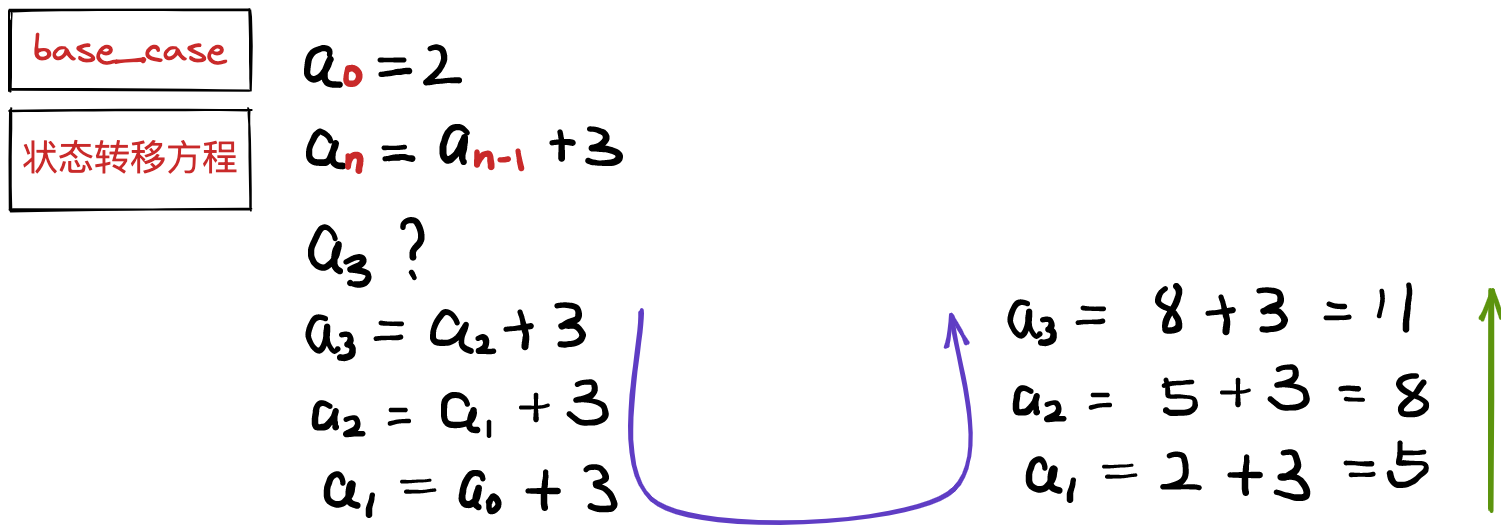
\includegraphics[width=.9\linewidth]{figures/dongtai.png}
\end{figure}

通俗来讲动态规划算法并不直接给出最终结果的求解表达式，而是通过找到问题规模之间的\cmagenta{状态转移方程}，借此不断缩小问题规模，逐渐迫近\cmagenta{base case}。所谓动态转移方程就是不同规模问题之间的关系，类似递推式。

{\bfseries \cgreen{动态规划解题方式}}

动态规划的解题方式通常分为两种：
\begin{enumerate}
    \item 通过定义递归方程解决，这是一种自顶向下的求解方式，通常这种方式会有很多重复计算过程，因此可以通过建立备忘录记录中间过程来进行优化。如上图紫色箭头方向。
\begin{lstlisting}
def func(n):
    if n == 0:
        return 2
    return func(n - 1) + 3
\end{lstlisting}
    \item 通过定义DP(Dynamic Programming)数组来求解，这是一种自底向上的求解方式。如上图绿色箭头方向。
\begin{lstlisting}
def func2(n):
    # 确定dp[i] 的含义
    # d[i] == func(i)
    # dp数组规模,规模与dp[i]的定义密切相关
    # 根据dp[i] 定义，func2(n) 对应dp[n]
    # 要使得dp[n] 合法，数组长度要为 n+1
    dp = [0] * (n + 1)
    # base_case
    dp[0] = 2
    # dp数组的遍历顺序
    # func(i) = func(i-1) + 3
    # dp[i] = dp[i-1] + 3
    for i in range(1, n + 1):
        dp[i] = dp[i - 1] + 3
    return dp[n]        
\end{lstlisting}
\end{enumerate}

{\bfseries \cgreen{重叠子问题}}

以斐波拉契数列为例：

\begin{lstlisting}
def fib(n):
    if n <= 2:
        return 1
    return fib(n-1) + fib(n-2)
\end{lstlisting}

我们来看一下递归的状态树：

\begin{figure}[htpb]
    \centering
    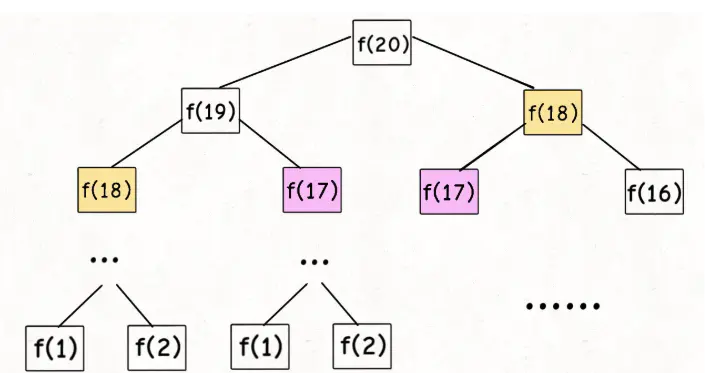
\includegraphics[width=.6\linewidth]{figures/tree.png}
\end{figure}

从状态树我们可以看到有很多重复计算的节点，重叠子问题导致了大量的重复计算。并且重复的计算量随着问题规模增大极速上升。此时的时间复杂度O$(2^n)$指数级，计算很慢。

因此，使用\cmagenta{备忘录}来减少重复计算非常有必要！我们可以通过建立一个备忘录memo，来记录中间节点的计算结果，避免重复计算，可以将时间复杂度直接降为O(n)线性复杂度，优化代码如下：

\begin{lstlisting}
# 使用一个字典存储计算过的fib(n)
# base_case 也可直接放入备忘录
# 字典以 n为键，fib(n) 为值
memo = {0: 0, 1: 1}

def fib(n):
    if n in memo:
        return memo[n]
    memo[n] = fib(n - 1) + fib(n - 2)
    return memo[n]
\end{lstlisting}

备忘录相当于为整个递归遍历树进行了一个剪枝操作。

使用dp数组自底向上来解不存在重叠子问题。空间开销为 O(n)
\begin{lstlisting}
def fib(n):
    dp = [0 for _ in range(n+1)]
    # 基础值，也就是baseline
    dp[1] = dp[2] = 1
    for i in range(3, n + 1):
        dp[i] = dp[i-1] + dp[i-2]
    return dp[n]
\end{lstlisting}

不难看出，每次计算新值只依赖前面两个值。因此我们可以使用两个变量来记录，而不使用dp数组，通过状态压缩减少空间开销。
\begin{lstlisting}
def fib(n):
    if n <= 2:
        return 1
    prev = 1
    curr = 1
    for i in range(3, n+1):
        sum = prev + curr
        prev = curr
        curr = sum
    return curr
\end{lstlisting}

当出现重叠子问题时，自顶向下的解法一需要备忘录来剪枝，自底向上的解法二需要状态压缩减少空间开销。

一般来说，自顶向下的方法如果不用备忘录剪枝，一般会超时。自底向上的方法不进行状态压缩一般也没事。

{\bfseries \cgreen{通用解题过程}}

动态规划没有标准的解题方法，即没有一个完全通用的解题方法。但在宏观上有通用的方法论：

下面的 k 表示多轮决策的第 k 轮：
\begin{enumerate}
    \item 问题分解，将原问题划分成几个子问题。一个子问题就是多轮决策的一个阶段。
    \item 找状态，选择合适的状态变量 S(k)。它需要具备描述多轮决策过程的演变，更像是决策可能的结果。
    \item 做决策，确定决策变量 u(k)。每一轮的决策就是每一轮可能的决策动作，即当前可以有哪些决策可以选择。
    \item 状态转移方程。这个步骤是动态规划最重要的核心，即 S(k+1)= uk(sk) 。
    \item 定目标。写出代表多轮决策目标的指标函数 V(k,n)，即最终需要达到的目标。
    \item 寻找目标的终止条件。
\end{enumerate}

{\bfseries \cgreen{状态转移方程}}

动态规划的解题核心就是找到状态转移方程，其实所谓的状态转移方程说白了就是数学上的递推方程，没有什么高大上的。就是通过最基础的问题，一步步递推出所需要的最终目标结果。只是在定义状态转移方程的含义时，有不同的定义方式，不同的定义方式会有不同的递推方程式，但是只要定义正确，都可以得到最终正确的结果。

通常状态转移方程定义过程：
\begin{enumerate}
    \item 明确当前可改变的状态有什么；
    \item 定义dp数组或者递归函数的具体含义；
    \item 明确每一步可以进行的选择有哪些；
    \item 编写递推方程，也就是状态转移方程；
    \item 明确baseline，也就是递推开始时的基础值是什么。
\end{enumerate}

{\bfseries \cgreen{海盗船装载问题}}

有一天海盗们截获了一艘装满各种各样宝物的货船，每一件都价值连城，宝物可分割。海盗船载重量为w，每件宝物的重量为$w_i$，价值$v_i$，海盗们该如何装载宝物，使运走宝物的价值最大呢？

\begin{table}[htpb]
    \centering
    \begin{tabular}{@{}ccccccccc@{}}
    \toprule
    \multicolumn{9}{c}{宝物清单}                \\ \midrule
    重量 & 4 & 10 & 7  & 11 & 3 & 5  & 14 & 2 \\
    价值 & 8 & 50 & 14 & 44 & 9 & 20 & 28 & 6 \\ \bottomrule
    \end{tabular}
\end{table}

记$m(i, w)$：表示载重量为w，现有i件宝物可装载，所能得到的最大价值。

\begin{itemize}
    \item 如果第 i 件宝物太重，装不到船上，那么前 i 件宝物价值等于前 i-1 件宝物价值，即 $m(i, w) = m(i-1, w)$；
    \item 如果第 i 件宝物可以加入到背包中，那么前 i 件宝物价值等于前 i-1 件宝物价值加上第 i 件宝物价值$w_i$，即 $m(i, w) = m(i-1, w-w_i) + v_i$。
\end{itemize}

因此，$m(i, w)$ 应该是$m(i-1, w)$ 和$m(i-1, w-w_i) + v_i$两者最大值，即

$m(i, w) = \mathrm{max}\{m(i-1, w), m(i-1, w-w_i) + v_i\}$

\begin{figure}[htpb]
    \centering
    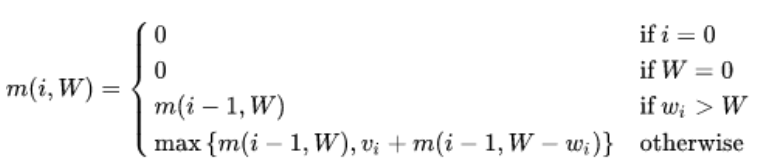
\includegraphics[width=.6\linewidth]{figures/ship.png}
\end{figure}

\begin{lstlisting}
goods = [None, {'w': 4,'v': 8}, {'w': 10,'v': 50}, {'w': 7,'v': 14}, {'w': 11,'v': 44}, {'w': 3,'v': 9}, {'w': 5,'v': 20}, {'w': 14,'v': 28}, {'w': 2,'v': 6}]
# 设置背包最大承重
max_w = 50
# 初始化二维表格m[(i, w)]，将表格中所有价值均初始化为0
# 表示前i个宝物中，最大重量w的组合，所得到的最大价值
# 当i或w为0时，价值为0
m = {(i, w): 0 for i in range(len(goods)) for w in range(max_w + 1)}
# 逐个填写二维表格
# 外层循环为 i个宝物，[1,9)的循环
# 内层循环为 重量w，[1, max_w+1)的循环
for i in range(1, len(goods)):
    for w in range(1, max_w + 1):
        if goods[i]['w'] > w:
            # 装不下第i个宝物，即不装第i个宝物
            m[(i, w)] = m[(i - 1, w)]
        else:
            # 装得下第i个宝物时，在不装第i个宝物与装第i个宝物这两种情况下，取最大价值
            m[(i, w)] = max(m[(i - 1, w)],
                            m[(i - 1, w - goods[i]['w'])] + goods[i]['v'])
# 输出结果
print(m[(len(goods) - 1, max_w)])
\end{lstlisting}

\section{回溯法}

\subsection{回溯法算法思想}

回溯法(探索与回溯法)是一种选优搜索法，按选优条件向前搜索，以达到目标。但当探索到某一步时，发现原先选择并不优或达不到目标，就退回一步重新选择，这种走不通就退回再走的技术为回溯法，而满足回溯条件的某个状态的点称为“回溯点”。

\begin{itemize}
    \item 有许多问题，当需要找出它的解集（全部解）或者要求回答什么解是满足某些约束条件的最优解时，往往要使用回溯法。
    \item 回溯法的基本做法是搜索或者有的组织穷尽搜索。它能避免搜索所有的可能性。即避免不必要的搜索。这种方法适用于解一些组合数相当大的问题。
    \item 回溯法在问题的解空间树中，按深度优先策略，从根结点出发搜索解空间树。算法搜索至解空间树的任意一点时，先判断该结点是否包含问题的解。如果肯定不包含（剪枝过程），则跳过对该结点为根的子树的搜索，逐层向其祖先结点回溯；否则，进入该子树，继续按深度优先策略搜索。
\end{itemize}

为了实现回溯，我们先弄明白以下两个问题：

\begin{enumerate}
    \item 首先应该明确问题的解空间。
    \item 其次是组织解空间以便它能用以被搜索到。
\end{enumerate}

\subsection{问题的解空间和空间树}

问题的解空间通常是在搜索问题的解的过程中动态产生的，这是回溯算法的一个重要特性。解空间的确定与我们对问题的描述有关。如何组织解空间的结构会直接影响对问题的求解效率。这是因为回溯方法的基本思想是通过搜索解空间来找到问题所要求的解。对于问题的解空间结构通常以树或图的形式表示，常用的两类典型的解空间树是子集树和排列树。

{\bfseries \cgreen{子集树}}

当所给的问题是从n个元素的集合S中找到S满足某种性质的子集时，相应的解空间树称为子集树。这类子集树通常有$2^n$个叶结点，遍历子集树的算法需要O$(2^n)$计算时间。

例如，定和子集问题：已知一个正实数的集合$P= {W_1,W_2, \cdots W_n}$和另一个正实数M。试求P的所有子集S，使得S中的数之和等于M。

这个问题的解可以表示成0/1数组${x_1,x_2,\cdots,x_n}$，依据$W_1$是否属于S， $x_1$分别取值1或0。故解空间中共有$2^n$个元素。它的树结构是一棵完整二叉树。 

{\bfseries \cgreen{排列树}}

当所给问题是确定n个元素满足某种性质的排列时，相应的解空间树称为排列树。排列树通常有n！个叶结点。因此，排列树需要O(n!)计算时间。















\newpage
\section{算法实例}
\begin{lstlisting}[caption = 求最大值]
a = input("请输入a：")
b = input("请输入b：")
a = float(a)
b = float(b)
if b < a:
    max = a
else:
    max = b
print(max)
\end{lstlisting}


\begin{lstlisting}[caption = 枚举算法]
k = int(input("请输入k："))
n = 10000
while n <= 30000:
    sub1 = int(n / 100)
    sub2 = int(n / 10) % 1000
    sub3 = n % 1000
    if sub1 % k == 0 and sub2 % k == 0 and sub3 % k == 0:
        print(n)
        n = n + 1
    else:
        n = n + 1
\end{lstlisting}


\begin{lstlisting}[caption = 谷角猜想]
n = int(input("请输入n："))
while n != 1:
    if n % 2 == 0:
        n = n / 2
    else:
        n = 3 * n + 1
print("猜想成功")
\end{lstlisting}

\newpage

\begin{lstlisting}[caption = 求平方根]
a = float(input("请输入a："))
x0 = float(input("请输入x0："))
x1 = 0.5 * (x0 + a / x0)
while abs(x1 - x0) > 0.000001:
    x0 = x1
    x1 = 0.5 * (x0 + a / x0)
print(x1)
\end{lstlisting}


\begin{lstlisting}[caption = 斐波那契数列]
n = int(input("请输入n："))

def fibonacci(n):
    if n <= 1:
        return 1
    return fibonacci(n - 1) + fibonacci(n - 2)

print(fibonacci(n))

def f(n):
    if n == 0:
        return 1
    return n * f(n - 1)

print(f(n))
\end{lstlisting}


\begin{lstlisting}[caption = 跳台阶问题]
n = int(input("请输入n："))

def f(n):
    if n <= 2:
        return n
    return f(n - 1) + f(n - 2)

print(f(n))
\end{lstlisting}


\newpage
\begin{lstlisting}[caption = 二分搜索]
lis = [1, 3, 4, 6, 7, 8, 10, 13, 14, 20, 22, 24, 30, 50, 80, 98, 100]

n = int(input('输入要查找的数:'))
left = 0
right = len(lis) - 1

while left <= right:    
    mid = (left + right) // 2  # 整除
    if n > lis[mid]:
        left = mid + 1
    elif n < lis[mid]:
        right = mid - 1
    else:
        print("要查找的数在数组中的索引为%s" % mid)
        break
else:
    print("没有这个数据")
\end{lstlisting}


\begin{lstlisting}[caption = 阶乘]
n = int(input("请输入n："))

def f(n):
    if n == 0:
        return 1
    return n * f(n - 1)

print(f(n))
\end{lstlisting}